\documentclass[12pt,nohyper]{tufte-handout}\usepackage[]{graphicx}\usepackage[]{color}
%% maxwidth is the original width if it is less than linewidth
%% otherwise use linewidth (to make sure the graphics do not exceed the margin)
\makeatletter
\def\maxwidth{ %
  \ifdim\Gin@nat@width>\linewidth
    \linewidth
  \else
    \Gin@nat@width
  \fi
}
\makeatother

\definecolor{fgcolor}{rgb}{0.345, 0.345, 0.345}
\newcommand{\hlnum}[1]{\textcolor[rgb]{0.686,0.059,0.569}{#1}}%
\newcommand{\hlstr}[1]{\textcolor[rgb]{0.192,0.494,0.8}{#1}}%
\newcommand{\hlcom}[1]{\textcolor[rgb]{0.678,0.584,0.686}{\textit{#1}}}%
\newcommand{\hlopt}[1]{\textcolor[rgb]{0,0,0}{#1}}%
\newcommand{\hlstd}[1]{\textcolor[rgb]{0.345,0.345,0.345}{#1}}%
\newcommand{\hlkwa}[1]{\textcolor[rgb]{0.161,0.373,0.58}{\textbf{#1}}}%
\newcommand{\hlkwb}[1]{\textcolor[rgb]{0.69,0.353,0.396}{#1}}%
\newcommand{\hlkwc}[1]{\textcolor[rgb]{0.333,0.667,0.333}{#1}}%
\newcommand{\hlkwd}[1]{\textcolor[rgb]{0.737,0.353,0.396}{\textbf{#1}}}%

\usepackage{framed}
\makeatletter
\newenvironment{kframe}{%
 \def\at@end@of@kframe{}%
 \ifinner\ifhmode%
  \def\at@end@of@kframe{\end{minipage}}%
  \begin{minipage}{\columnwidth}%
 \fi\fi%
 \def\FrameCommand##1{\hskip\@totalleftmargin \hskip-\fboxsep
 \colorbox{shadecolor}{##1}\hskip-\fboxsep
     % There is no \\@totalrightmargin, so:
     \hskip-\linewidth \hskip-\@totalleftmargin \hskip\columnwidth}%
 \MakeFramed {\advance\hsize-\width
   \@totalleftmargin\z@ \linewidth\hsize
   \@setminipage}}%
 {\par\unskip\endMakeFramed%
 \at@end@of@kframe}
\makeatother

\definecolor{shadecolor}{rgb}{.97, .97, .97}
\definecolor{messagecolor}{rgb}{0, 0, 0}
\definecolor{warningcolor}{rgb}{1, 0, 1}
\definecolor{errorcolor}{rgb}{1, 0, 0}
\newenvironment{knitrout}{}{} % an empty environment to be redefined in TeX

\usepackage{alltt}
\usepackage[T1]{fontenc}
\usepackage[latin9]{inputenc}
\usepackage{wrapfig}
\usepackage{longtable}
\usepackage{hyperref}
\usepackage{graphicx}
\usepackage[space]{grffile}

\makeatletter
%%%%%%%%%%%%%%%%%%%%%%%%%%%%%% Textclass specific LaTeX commands.
\newcommand{\Rcode}[1]{{\texttt{#1}}}
\newcommand{\Robject}[1]{{\texttt{#1}}}
\newcommand{\Rcommand}[1]{{\texttt{#1}}}
\newcommand{\Rfunction}[1]{{\texttt{#1}}}
\newcommand{\Rfunarg}[1]{{\textit{#1}}}
\newcommand{\Rpackage}[1]{{\textit{#1}}}
\newcommand{\Rmethod}[1]{{\textit{#1}}}
\newcommand{\Rclass}[1]{{\textit{#1}}}

\makeatother
\IfFileExists{upquote.sty}{\usepackage{upquote}}{}
\begin{document}



\centerline{\Large\bf Introductory Statistics Homework Short Report for Topic 06}
\centerline{\bf Comparison among Sections}
\centerline{\bf }

\section{Overview}


\begin{marginfigure}
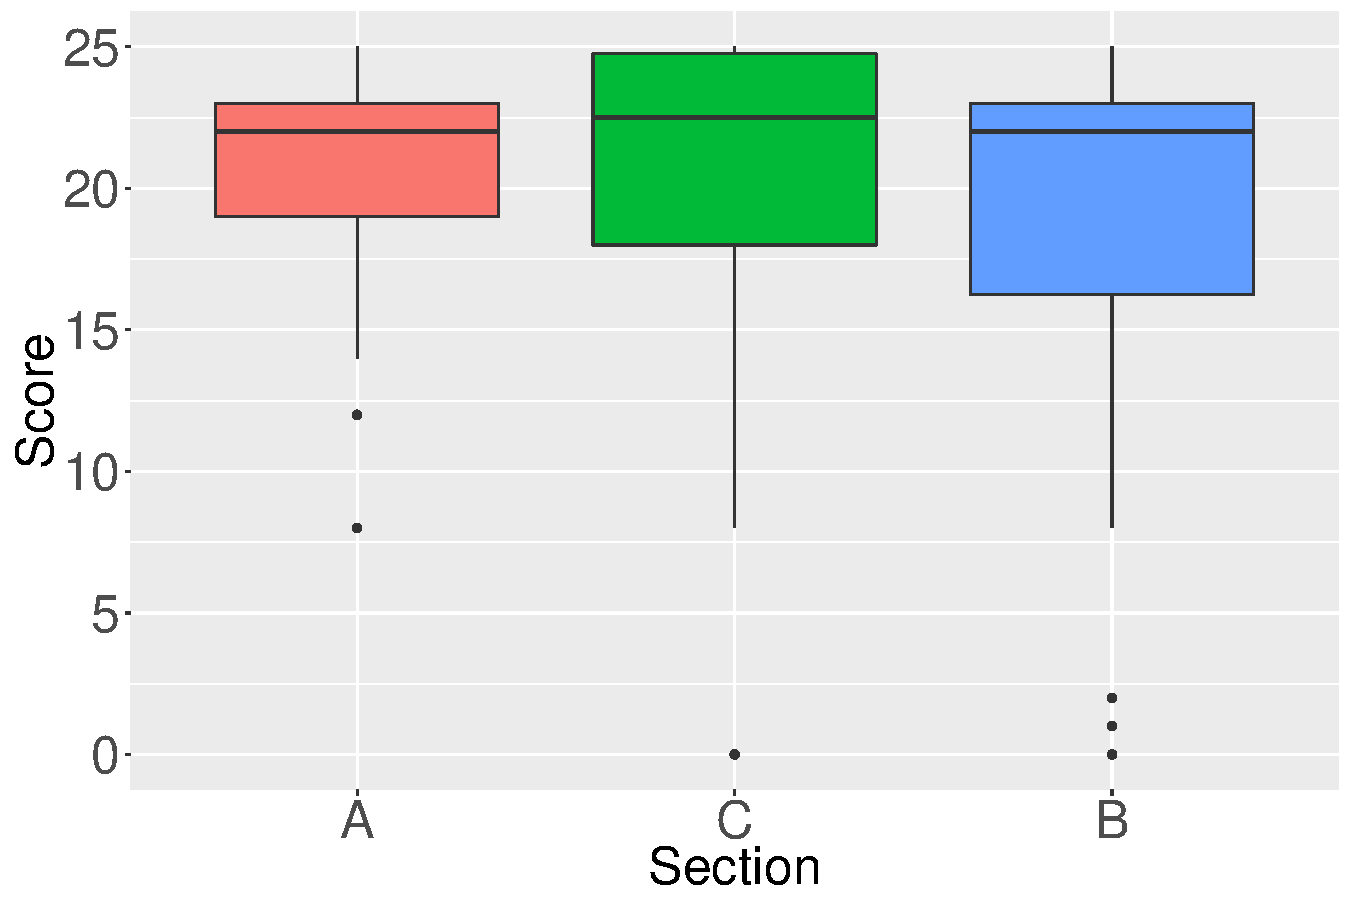
\includegraphics[width=0.95\linewidth]{Topic06_boxplot_score}
\caption{\label{fig:boxplot-score}Boxplot for the overall scores by section. The highest median comes from Section AB,CD.}
\end{marginfigure}

The homework results that will be compared are Topic06.AB.csv, Topic06.CD.csv.

Figure \ref{fig:boxplot-score} shows the side-by-side boxplots
for the overall scores by section.
Table \ref{tab:Oset} gives the average percentages correct for
each learning outcome by section. Any percentages below 80
will be marked red.

\marginnote{

 \bigskip{} 

 \bigskip{} 

} \marginnote{Learning objectives in this topic:

 \bigskip{} 

Use standardizing to determine how many standard deviations an observation is away from the mean value.

 \bigskip{} 

Use z-scores to compare observations for different quantitative variables.

 \bigskip{} 

Explain how standardizing affects the shape, center, and variability of the distribution of a quantitative variable.

 \bigskip{} 

Determine which quantitative variables could be modeled using the normal distribution by interpreting graphical representations of the variable.

 \bigskip{} 

Apply the 68-95-99.

 \bigskip{} 

Find percentile or area values for any given observation from a normal distribution.

 \bigskip{} 

Find the value of an observation when given a percentile or area value from the normal distribution.

 \bigskip{} 

}
% latex table generated in R 3.2.2 by xtable 1.8-0 package
% Mon Nov 23 01:11:02 2015
\begin{longtable}{rll}
  \hline
 & CD & AB \\ 
  \hline
D & \color{red}{72} & \color{red}{61} \\ 
  B & \color{red}{31} & \color{red}{38} \\ 
  A & \color{red}{25.5} & \color{red}{23} \\ 
  G & \color{red}{26} & \color{red}{21.5} \\ 
  C & \color{red}{22} & \color{red}{22} \\ 
  F & \color{red}{19.2} & \color{red}{20.8} \\ 
  E & \color{red}{20.67} & \color{red}{16.67} \\ 
   \hline
\hline
\caption{Average percentages correct for each learning outcome by section. Learning outcomes are sorted by the average percentages correct of all sections, from the highest to the lowest.} 
\label{tab:Oset}
\end{longtable}


\subsection{Problematic question sets}

% latex table generated in R 3.2.2 by xtable 1.8-0 package
% Mon Nov 23 01:11:02 2015
\begin{longtable}{ccclc}
  \hline
ID & LO & Qset & Name & CrtPct \\ 
  \hline
  1 & A & A & 1 & 46.15 \\ 
    2 & A & A & 2 & 54.17 \\ 
    3 & A & A & 3 & 36.36 \\ 
    4 & A & A & 4 & 46.43 \\ 
   &  &  &  &  \\ 
    5 & A & B & 1 & 50.00 \\ 
    6 & A & B & 2 & 50.00 \\ 
    7 & A & B & 3 & 52.38 \\ 
    8 & A & B & 4 & 52.38 \\ 
   &  &  &  &  \\ 
    9 & A & C & 1 & 0.00 \\ 
   10 & A & C & 2 & 0.00 \\ 
   11 & A & C & 3 & 0.00 \\ 
   12 & A & C & 4 & 0.00 \\ 
   &  &  &  &  \\ 
   13 & A & D & 1 & 0.00 \\ 
   14 & A & D & 2 & 0.00 \\ 
   15 & A & D & 3 & 0.00 \\ 
   16 & A & D & 4 & 0.00 \\ 
   &  &  &  &  \\ 
   17 & B & E & compare1 & 41.00 \\ 
   &  &  &  &  \\ 
   18 & B & F & compare2 & 28.00 \\ 
   &  &  &  &  \\ 
   19 & C & G & 1 & 20.00 \\ 
   &  &  &  &  \\ 
   20 & C & H & 1 & 24.00 \\ 
   &  &  &  &  \\ 
   21 & D & I & feet & 73.91 \\ 
   22 & D & I & lowtemp & 70.37 \\ 
   &  &  &  &  \\ 
   23 & D & J & gain & 60.71 \\ 
   24 & D & J & mpg & 80.00 \\ 
   25 & D & J & blowhole & 64.29 \\ 
   26 & D & J & CDs & 52.94 \\ 
   &  &  &  &  \\ 
   27 & E & K & whale1 & 25.71 \\ 
   28 & E & K & whale2 & 6.06 \\ 
   29 & E & K & whale3 & 14.71 \\ 
   30 & E & K & cow1 & 17.65 \\ 
   31 & E & K & cow2 & 7.89 \\ 
   32 & E & K & cow3 & 14.29 \\ 
   33 & E & K & bulbs1 & 22.58 \\ 
   34 & E & K & bulbs2 & 9.68 \\ 
   35 & E & K & bulbs3 & 13.89 \\ 
   &  &  &  &  \\ 
   36 & E & L & heights1 & 15.79 \\ 
   37 & E & L & heights2 & 15.79 \\ 
   38 & E & L & heights3 & 38.46 \\ 
   39 & E & L & mm1 & 3.33 \\ 
   40 & E & L & mm2 & 26.67 \\ 
   41 & E & L & mm3 & 17.95 \\ 
   42 & E & L & IQ1 & 36.36 \\ 
   43 & E & L & IQ2 & 28.00 \\ 
   44 & E & L & IQ3 & 21.43 \\ 
   &  &  &  &  \\ 
   45 & F & M & mm1 & 40.74 \\ 
   46 & F & M & Bulb1 & 16.67 \\ 
   47 & F & M & IQ1 & 31.58 \\ 
   48 & F & M & Whale1 & 41.18 \\ 
   49 & F & M & Cow1 & 10.53 \\ 
   &  &  &  &  \\ 
   50 & F & N & mm2 & 22.22 \\ 
   51 & F & N & Bulb2 & 5.88 \\ 
   52 & F & N & IQ2 & 27.27 \\ 
   53 & F & N & Whale2 & 26.32 \\ 
   54 & F & N & Cow2 & 12.50 \\ 
   &  &  &  &  \\ 
   55 & F & O & mm3 & 20.00 \\ 
   56 & F & O & Bulb3 & 14.29 \\ 
   57 & F & O & IQ3 & 8.00 \\ 
   58 & F & O & Whale3 & 24.00 \\ 
   59 & F & O & Cow3 & 23.81 \\ 
   &  &  &  &  \\ 
   60 & F & P & mm4 & 8.70 \\ 
   61 & F & P & Bulb4 & 5.88 \\ 
   62 & F & P & IQ4 & 20.00 \\ 
   63 & F & P & Whale4 & 5.26 \\ 
   64 & F & P & Cow4 & 14.29 \\ 
   &  &  &  &  \\ 
   65 & F & Q & mm5 & 27.78 \\ 
   66 & F & Q & Bulb5 & 26.32 \\ 
   67 & F & Q & IQ5 & 10.53 \\ 
   68 & F & Q & Whale5 & 27.27 \\ 
   69 & F & Q & Cow5 & 24.24 \\ 
   &  &  &  &  \\ 
   70 & G & R & mm1 & 33.33 \\ 
   71 & G & R & Bulb1 & 22.73 \\ 
   72 & G & R & IQ1 & 16.67 \\ 
   73 & G & R & Whale1 & 24.00 \\ 
   74 & G & R & Cow1 & 20.00 \\ 
   &  &  &  &  \\ 
   75 & G & S & mm2 & 35.71 \\ 
   76 & G & S & Bulb2 & 23.53 \\ 
   77 & G & S & IQ2 & 13.64 \\ 
   78 & G & S & Whale2 & 27.78 \\ 
   79 & G & S & Cow2 & 26.67 \\ 
   &  &  &  &  \\ 
   80 & G & T & mm3 & 18.18 \\ 
   81 & G & T & Bulb3 & 31.25 \\ 
   82 & G & T & IQ3 & 8.00 \\ 
   83 & G & T & Whale3 & 12.50 \\ 
   84 & G & T & Cow3 & 14.29 \\ 
   &  &  &  &  \\ 
   85 & G & U & mm4 & 16.67 \\ 
   86 & G & U & Bulb4 & 35.00 \\ 
   87 & G & U & IQ4 & 33.33 \\ 
   88 & G & U & Whale4 & 21.43 \\ 
   89 & G & U & Cow4 & 33.33 \\ 
   \hline
\hline
\caption{Question sets with any question correct percentage less than 80.} 
\label{tab:summary_question}
\end{longtable}
% latex table generated in R 3.2.2 by xtable 1.8-0 package
% Mon Nov 23 01:11:02 2015
\begin{longtable}{ccclcl}
  \hline
ID & LO & Qset & Name & CrtPct & Flag \\ 
  \hline
  1 & A & A & 1 & 46.15 &  \\ 
    2 & A & A & 2 & 54.17 & * \\ 
    3 & A & A & 3 & 36.36 & * \\ 
    4 & A & A & 4 & 46.43 &  \\ 
   &  &  &  &  &  \\ 
   23 & D & J & gain & 60.71 & * \\ 
   24 & D & J & mpg & 80.00 & * \\ 
   25 & D & J & blowhole & 64.29 & * \\ 
   26 & D & J & CDs & 52.94 & * \\ 
   &  &  &  &  &  \\ 
   27 & E & K & whale1 & 25.71 & * \\ 
   28 & E & K & whale2 & 6.06 & * \\ 
   29 & E & K & whale3 & 14.71 &  \\ 
   30 & E & K & cow1 & 17.65 &  \\ 
   31 & E & K & cow2 & 7.89 & * \\ 
   32 & E & K & cow3 & 14.29 &  \\ 
   33 & E & K & bulbs1 & 22.58 & * \\ 
   34 & E & K & bulbs2 & 9.68 & * \\ 
   35 & E & K & bulbs3 & 13.89 &  \\ 
   &  &  &  &  &  \\ 
   36 & E & L & heights1 & 15.79 & * \\ 
   37 & E & L & heights2 & 15.79 & * \\ 
   38 & E & L & heights3 & 38.46 & * \\ 
   39 & E & L & mm1 & 3.33 & * \\ 
   40 & E & L & mm2 & 26.67 & * \\ 
   41 & E & L & mm3 & 17.95 & * \\ 
   42 & E & L & IQ1 & 36.36 & * \\ 
   43 & E & L & IQ2 & 28.00 & * \\ 
   44 & E & L & IQ3 & 21.43 & * \\ 
   &  &  &  &  &  \\ 
   45 & F & M & mm1 & 40.74 & * \\ 
   46 & F & M & Bulb1 & 16.67 & * \\ 
   47 & F & M & IQ1 & 31.58 & * \\ 
   48 & F & M & Whale1 & 41.18 & * \\ 
   49 & F & M & Cow1 & 10.53 & * \\ 
   &  &  &  &  &  \\ 
   50 & F & N & mm2 & 22.22 & * \\ 
   51 & F & N & Bulb2 & 5.88 & * \\ 
   52 & F & N & IQ2 & 27.27 & * \\ 
   53 & F & N & Whale2 & 26.32 & * \\ 
   54 & F & N & Cow2 & 12.50 &  \\ 
   &  &  &  &  &  \\ 
   55 & F & O & mm3 & 20.00 &  \\ 
   56 & F & O & Bulb3 & 14.29 &  \\ 
   57 & F & O & IQ3 & 8.00 & * \\ 
   58 & F & O & Whale3 & 24.00 & * \\ 
   59 & F & O & Cow3 & 23.81 & * \\ 
   &  &  &  &  &  \\ 
   65 & F & Q & mm5 & 27.78 & * \\ 
   66 & F & Q & Bulb5 & 26.32 & * \\ 
   67 & F & Q & IQ5 & 10.53 & * \\ 
   68 & F & Q & Whale5 & 27.27 & * \\ 
   69 & F & Q & Cow5 & 24.24 &  \\ 
   &  &  &  &  &  \\ 
   70 & G & R & mm1 & 33.33 & * \\ 
   71 & G & R & Bulb1 & 22.73 &  \\ 
   72 & G & R & IQ1 & 16.67 & * \\ 
   73 & G & R & Whale1 & 24.00 &  \\ 
   74 & G & R & Cow1 & 20.00 &  \\ 
   &  &  &  &  &  \\ 
   75 & G & S & mm2 & 35.71 & * \\ 
   76 & G & S & Bulb2 & 23.53 &  \\ 
   77 & G & S & IQ2 & 13.64 & * \\ 
   78 & G & S & Whale2 & 27.78 &  \\ 
   79 & G & S & Cow2 & 26.67 &  \\ 
   &  &  &  &  &  \\ 
   80 & G & T & mm3 & 18.18 &  \\ 
   81 & G & T & Bulb3 & 31.25 & * \\ 
   82 & G & T & IQ3 & 8.00 & * \\ 
   83 & G & T & Whale3 & 12.50 & * \\ 
   84 & G & T & Cow3 & 14.29 & * \\ 
   &  &  &  &  &  \\ 
   85 & G & U & mm4 & 16.67 & * \\ 
   86 & G & U & Bulb4 & 35.00 & * \\ 
   87 & G & U & IQ4 & 33.33 & * \\ 
   88 & G & U & Whale4 & 21.43 &  \\ 
   89 & G & U & Cow4 & 33.33 & * \\ 
   \hline
\hline
\caption{Question sets with range greater than 15.} 
\label{tab:summary_question}
\end{longtable}


\end{document}
